\documentclass[preview, tikz]{standalone}
\def\kochsegment#1#2{--++(#1:#2) -- ++(#1+60:#2) -- ++(#1-60:#2) -- ++(#1:#2)}
\begin{document}
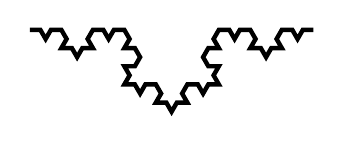
\begin{tikzpicture}[xscale=1.2, yscale=-1.2]
	\draw[ultra thick] (0, 0)
		\kochsegment{0}{1/9}
		\kochsegment{60}{1/9}
		\kochsegment{-60}{1/9}
		\kochsegment{0}{1/9}
		
		\kochsegment{60}{1/9}
		\kochsegment{120}{1/9}
		\kochsegment{0}{1/9}
		\kochsegment{60}{1/9}
		
		\kochsegment{-60}{1/9}
		\kochsegment{0}{1/9}
		\kochsegment{-120}{1/9}
		\kochsegment{-60}{1/9}
		
		\kochsegment{0}{1/9}
		\kochsegment{60}{1/9}
		\kochsegment{-60}{1/9}
		\kochsegment{0}{1/9}
	;
\end{tikzpicture}
\end{document}